\documentclass{standalone}
\usepackage{tikz}

\usetikzlibrary{calc,intersections}


\begin{document}

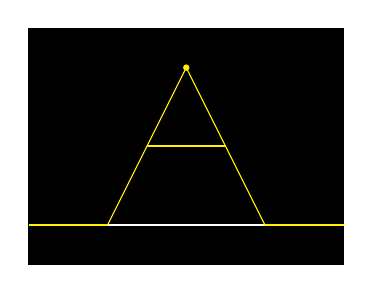
\begin{tikzpicture}
  \coordinate (light) at (0,2);
  \coordinate (P1) at (-0.5,1);
  \coordinate (P2) at (0.5,1);

  \draw[fill=black] (-2,-0.5) rectangle (2,2.5);
  \draw[white!10,thick,name path=wall] (-2,0) -- (2,0);
  \draw[yellow,thick] (P1) -- (P2);
  \draw[fill=yellow] (light) circle [radius=0.05cm];

  \begin{scope}
    \path[clip] (-2,0) rectangle (2,2);

    \draw[yellow] (light) -- ($ (light) ! 2 ! (P1) $);
    \draw[yellow] (light) -- ($ (light) ! 2 ! (P2) $);
  \end{scope}

  \path[name path=ray1] (light) -- ($ (light) ! 2 ! (P1) $);
  \path[name path=ray2] (light) -- ($ (light) ! 2 ! (P2) $);

  \draw[thick,yellow,name intersections={of=wall and ray1,by=h1}] (-2,0) -- (h1);
  \draw[thick,yellow,name intersections={of=wall and ray2,by=h2}] (2,0) -- (h2);
\end{tikzpicture}

\end{document}